\documentclass[aspectratio=169]{beamer}
\input{definitions/macros}
\input{definitions/letterfonts}

\usepackage{appendixnumberbeamer}
\usepackage{tikz}
\usepackage{tikz-cd}
\usepackage{graphicx}
\usetikzlibrary{positioning,quotes,calc,patterns,babel}
\usetikzlibrary{shapes.geometric,calc, decorations.pathmorphing, arrows.meta, overlay-beamer-styles}
\usetheme[progressbar=frametitle, block=fill]{metropolis}

\title{Cluster algebras and where to find them}
\date{June 28, 2024}
\author{Wannes Malfait}
\institute{Vrije Universiteit Brussel}


\begin{document}
\maketitle
\section{Combinatorics $\to$ algebra}
\begin{frame}{The goal}
	\uncover<2>{
		\begin{center}
			Triangulations
		\end{center}
	}
	\begin{center}
		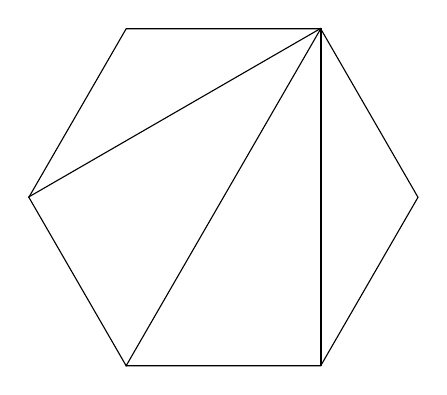
\begin{tikzpicture}
			\node[name=h,shape=regular polygon, regular polygon sides = 6, draw, inner sep = 10ex] {};
			\only<2>{
				\draw (h.corner 1) -- (h.corner 3);
				\draw (h.corner 1) -- (h.corner 4);
				\draw (h.corner 1) -- (h.corner 5);
			}
		\end{tikzpicture}
	\end{center}
\end{frame}

\begin{frame}
	\frametitle{Triangulations of a polygon}
	\begin{columns}[c]
		\begin{column}{0.4\textwidth}
			Observations:
			\begin{itemize}
				\item Flipping a diagonal
				      %
				\item<5-> Ptolomy's rule\uncover<6->{:
						\begin{equation*}
							{\color{red} |ac| \cdot |b d|} = |ab| \cdot |cd| + |ad| \cdot |bc|
						\end{equation*}}

				\item<7> Sides $\neq$ diagonals
			\end{itemize}
		\end{column}
		\begin{column}{0.6\textwidth}
			\begin{center}
				\begin{tikzpicture}
					\node[name=h,shape=regular polygon, regular polygon sides = 6, draw, alt=<{2,3,5,6}>{gray}{mDarkTeal}, minimum size = 30ex] {};
					\draw (h.corner 1) -- (h.corner 3);
					\only<1,2,5,6> {
						\draw[alt=<{2,5,6}>{dashed, red}{solid, mDarkTeal}] (h.corner 1) -- (h.corner 4);
					}
					\only<3->{
						\draw[alt=<{3,5,6}>{dashed, red}{solid, mDarkTeal}] (h.corner 3) -- (h.corner 5);
					}
					\uncover<6>{
						\node[circle, draw, minimum size = 30ex] {};
					}
					\only<{2,3,5,6}>{
						\draw (h.corner 3) -- (h.corner 4);
						\draw (h.corner 4) -- (h.corner 5);
					}
					\draw (h.corner 1) -- (h.corner 5);
					\uncover<{5,6}>{
						\node[above] at (h.corner 1) {a};
						\node[left] at (h.corner 3) {b};
						\node[below] at (h.corner 4) {c};
						\node[below] at (h.corner 5) {d};
					}
				\end{tikzpicture}
			\end{center}
		\end{column}
	\end{columns}
\end{frame}

\begin{frame}
	\frametitle{The cluster algebra}

	\begin{equation*}
		\{\text{ sides }\} \cup \{ \text{ diagonals }\} \longrightarrow \{x_1, \dotsc, x_m\}
	\end{equation*}
	\pause
	\begin{itemize}
		\item Flip $\leadsto$ mutate a variable\pause
		      \begin{equation*}
			      x_i' = \frac{x_a x_c + x_b x_d}{x_i}
		      \end{equation*}
		      \begin{equation*}
			      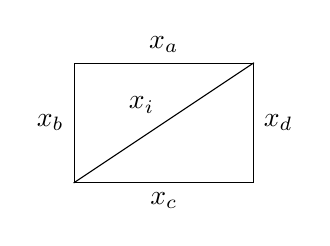
\begin{tikzpicture}[baseline]
				      \node[name=r, draw, inner sep = 5ex, xscale = 1.5]     {};
				      \node[above] at  (r.north) {$x_a$};
				      \node[left]  at  (r.west) {$x_b$};
				      \node[below] at  (r.south) {$x_c$};
				      \node[right] at  (r.east) {$x_d$};
				      \draw (r.south west) edge["$x_i$"] (r.north east);
			      \end{tikzpicture}
			      \qquad\longrightarrow\qquad
			      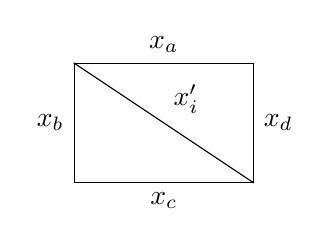
\begin{tikzpicture}[baseline]
				      \node[name=r, draw, inner sep = 5ex, xscale = 1.5]        {};
				      \node[above] at  (r.north) {$x_a$};
				      \node[left]  at  (r.west) {$x_b$};
				      \node[below] at  (r.south) {$x_c$};
				      \node[right] at  (r.east) {$x_d$};
				      \draw (r.north west) edge["$x_i'$"] (r.south east);
			      \end{tikzpicture}
		      \end{equation*}
		      \pause
		\item \emph{Cluster algebra} $=$ subalgebra of $\mathbb{C}(x_1, \dotsc, x_m)$ generated by cluster variables.
	\end{itemize}

\end{frame}

\begin{frame}
	\frametitle{The quiver}

	\begin{center}
		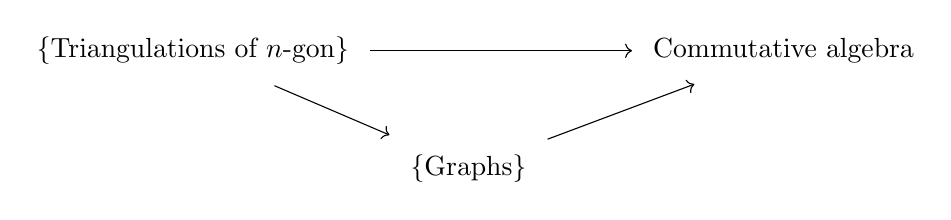
\begin{tikzpicture}
			\node[outer sep=1ex] (triangulations) at (-3.5,0) {\{Triangulations of $n$-gon\}};
			\node[outer sep=1ex] (clusteralgebra) at (4, 0) {Commutative algebra};
			\draw[->, alt=<1>{solid}{dashed}] (triangulations) -- (clusteralgebra);
			\uncover<2->{
				\node[outer sep=1ex] (graph) at (0,-1.5) {\{Graphs\}};
				\draw[->] (triangulations) -- (graph);
				\draw[->] (graph) -- (clusteralgebra);
			}
		\end{tikzpicture}
	\end{center}
	\uncover<3->{
		\begin{center}
			\begin{tikzpicture}[
					R/.style = {rectangle, alt=<{3,6}>{fill=none}{fill=mDarkTeal}, inner sep=0.7ex},
					B/.style = {circle, alt=<{3,6}>{fill=none}{fill=mDarkTeal}, inner sep=0.7ex},
					every edge/.style= {draw, mDarkTeal},
					baseline
				]
				\coordinate (center) at (0,0);
				\def\radius{10ex}

				% points on the circle
				\begin{scope}[rotate=120]
					\path (center) ++(0:\radius) coordinate (A);
					\path (center) ++(60:\radius) coordinate (B);
					\path (center) ++(120:\radius) coordinate (C);
					\path (center) ++(180:\radius) coordinate (D);
					\path (center) ++(240:\radius) coordinate (E);
					\path (center) ++(300:\radius) coordinate (F);
				\end{scope}

				% Sides with frozen verts
				\begin{scope}[nodes=R]
					\path (A) edge node (AB) {} (B);
					\path (B) edge node (BC) {} (C);
					\path (C) edge node (CD) {} (D);
					\path (D) edge node (DE) {} (E);
					\path (E) edge node (EF) {} (F);
					\path (F) edge node (AF) {} (A);
				\end{scope}

				% Diagonals with exchangeable verts
				\begin{scope}[nodes=B]
					\path (A) edge node (AC) {} (C);
					\path (A) edge node (AD) {} (D);
					\path (D) edge node (DF) {} (F);
					% \path (A) edge node (AG) {} (G);
					% \path (D) edge node (DG) {} (G);
					% \path (E) edge node (EG) {} (G);
				\end{scope}

				% Quiver edges
				\begin{scope}[every edge/.style={alt=<{3,4,6}>{draw=none}{draw}, -Latex,mDarkTeal,line width=0.2ex}]
					\path (AB) edge (AC);
					\path (AC) edge (BC);
					\path (AC) edge (AD);
					\path (CD) edge (AC);
					\path (AD) edge (CD);
					\path (AD) edge (AF);
					\path (AF) edge (DF);
					\path (DF) edge (AD);
					\path (DF) edge (EF);
					\path (DE) edge (DF);
					% \path (AD) edge (AG);
					% \path (DG) edge (AD);
					% \path (AG) edge (DG);
					% \path (AG) edge (HA);
					% \path (GH) edge (AG);
					% \path (DE) edge (DG);
					% \path (DG) edge (EG);
					% \path (EG) edge (FG);
					% \path (EF) edge (EG);
				\end{scope}
			\end{tikzpicture}
			\only<6>{
				$\qquad \longrightarrow \qquad$
				\begin{tikzpicture}[
						R/.style = {rectangle, fill=mDarkTeal, inner sep=0.7ex},
						B/.style = {circle, fill=mDarkTeal, inner sep=0.7ex},
						every edge/.style= {draw=none},
						baseline
					]
					\coordinate (center) at (0,0);
					\def\radius{10ex}

					% points on the circle
					\begin{scope}[rotate=120]
						\path (center) ++(0:\radius) coordinate (A);
						\path (center) ++(60:\radius) coordinate (B);
						\path (center) ++(120:\radius) coordinate (C);
						\path (center) ++(180:\radius) coordinate (D);
						\path (center) ++(240:\radius) coordinate (E);
						\path (center) ++(300:\radius) coordinate (F);
					\end{scope}

					% Sides with frozen verts
					\begin{scope}[nodes=R]
						\path (A) edge node (AB) {} (B);
						\path (B) edge node (BC) {} (C);
						\path (C) edge node (CD) {} (D);
						\path (D) edge node (DE) {} (E);
						\path (E) edge node (EF) {} (F);
						\path (F) edge node (AF) {} (A);
					\end{scope}

					% Diagonals with exchangeable verts
					\begin{scope}[nodes=B]
						\path (A) edge node (AC) {} (C);
						\path (A) edge node (AD) {} (D);
						\path (D) edge node (DF) {} (F);
						% \path (A) edge node (AG) {} (G);
						% \path (D) edge node (DG) {} (G);
						% \path (E) edge node (EG) {} (G);
					\end{scope}

					% Quiver edges
					\begin{scope}[every edge/.style={draw, -Latex,mDarkTeal,line width=0.2ex}]
						\path (AB) edge (AC);
						\path (AC) edge (BC);
						\path (AC) edge (AD);
						\path (CD) edge (AC);
						\path (AD) edge (CD);
						\path (AD) edge (AF);
						\path (AF) edge (DF);
						\path (DF) edge (AD);
						\path (DF) edge (EF);
						\path (DE) edge (DF);
						% \path (AD) edge (AG);
						% \path (DG) edge (AD);
						% \path (AG) edge (DG);
						% \path (AG) edge (HA);
						% \path (GH) edge (AG);
						% \path (DE) edge (DG);
						% \path (DG) edge (EG);
						% \path (EG) edge (FG);
						% \path (EF) edge (EG);
					\end{scope}
				\end{tikzpicture}
			}
		\end{center}
	}
\end{frame}

\begin{frame}
	\frametitle{Quiver Mutation}
	\begin{columns}[c]

		\begin{column}{0.4\textwidth}
			\begin{center}

				\begin{tikzpicture}[
						R/.style = {rectangle, fill=none, inner sep=0.7ex},
						B/.style = {circle, fill=none, inner sep=0.7ex},
						every edge/.style= {draw, mDarkTeal},
						baseline
					]
					\coordinate (center) at (0,0);
					\def\radius{8ex}

					% points on the circle
					\begin{scope}[rotate=120]
						\path (center) ++(0:\radius) coordinate (A);
						\path (center) ++(60:\radius) coordinate (B);
						\path (center) ++(120:\radius) coordinate (C);
						\path (center) ++(180:\radius) coordinate (D);
						\path (center) ++(240:\radius) coordinate (E);
						\path (center) ++(300:\radius) coordinate (F);
					\end{scope}

					% Sides with frozen verts
					\begin{scope}[nodes=R]
						\path (A) edge node (AB) {} (B);
						\path (B) edge node (BC) {} (C);
						\path (C) edge node (CD) {} (D);
						\path (D) edge node (DE) {} (E);
						\path (E) edge node (EF) {} (F);
						\path (F) edge node (AF) {} (A);
					\end{scope}

					% Diagonals with exchangeable verts
					\begin{scope}[nodes=B]
						\path (A) edge node (AC) {} (C);
						\path (A) edge node (AD) {} (D);
						\path (D) edge node (DF) {} (F);
					\end{scope}
				\end{tikzpicture}
				\uncover<2->{
					\begin{equation*}
						\downarrow
					\end{equation*}

					\begin{tikzpicture}[
							R/.style = {rectangle, fill=none, inner sep=0.7ex},
							B/.style = {circle, fill=none, inner sep=0.7ex},
							every edge/.style= {draw, mDarkTeal},
							baseline
						]
						\coordinate (center) at (0,0);
						\def\radius{8ex}

						% points on the circle
						\begin{scope}[rotate=120]
							\path (center) ++(0:\radius) coordinate (A);
							\path (center) ++(60:\radius) coordinate (B);
							\path (center) ++(120:\radius) coordinate (C);
							\path (center) ++(180:\radius) coordinate (D);
							\path (center) ++(240:\radius) coordinate (E);
							\path (center) ++(300:\radius) coordinate (F);
						\end{scope}

						% Sides with frozen verts
						\begin{scope}[nodes=R]
							\path (A) edge node (AB) {} (B);
							\path (B) edge node (BC) {} (C);
							\path (C) edge node (CD) {} (D);
							\path (D) edge node (DE) {} (E);
							\path (E) edge node (EF) {} (F);
							\path (F) edge node (AF) {} (A);
						\end{scope}

						% Diagonals with exchangeable verts
						\begin{scope}[nodes=B]
							\path (A) edge node (AC) {} (C);
							\path (C) edge node (CF) {} (F);
							\path (D) edge node (DF) {} (F);
							% \path (A) edge node (AG) {} (G);
							% \path (D) edge node (DG) {} (G);
							% \path (E) edge node (EG) {} (G);
						\end{scope}
					\end{tikzpicture}
				}
			\end{center}
		\end{column}

		\begin{column}{0.2\textwidth}
			\uncover<3>{
				\begin{equation*}
					x_i' = \frac{1}{x_i}\Bigl( \prod_{i \to j} x_j + \prod_{j \to i} x_j\Bigr)
				\end{equation*}
			}
		\end{column}

		\begin{column}{0.4\textwidth}
			\begin{center}

				\begin{tikzpicture}[
						R/.style = {rectangle, fill=mDarkTeal, inner sep=0.7ex},
						B/.style = {circle, fill=mDarkTeal, inner sep=0.7ex},
						every edge/.style= {draw=none},
						baseline
					]
					\coordinate (center) at (0,0);
					\def\radius{8ex}

					% points on the circle
					\begin{scope}[rotate=120]
						\path (center) ++(0:\radius) coordinate (A);
						\path (center) ++(60:\radius) coordinate (B);
						\path (center) ++(120:\radius) coordinate (C);
						\path (center) ++(180:\radius) coordinate (D);
						\path (center) ++(240:\radius) coordinate (E);
						\path (center) ++(300:\radius) coordinate (F);
					\end{scope}

					% Sides with frozen verts
					\begin{scope}[nodes=R]
						\path (A) edge node (AB) {} (B);
						\path (B) edge node (BC) {} (C);
						\path (C) edge node (CD) {} (D);
						\path (D) edge node (DE) {} (E);
						\path (E) edge node (EF) {} (F);
						\path (F) edge node (AF) {} (A);
					\end{scope}

					% Diagonals with exchangeable verts
					\begin{scope}[nodes=B]
						\path (A) edge node (AC) {} (C);
						\path (A) edge node (AD) {} (D);
						\path (D) edge node (DF) {} (F);
					\end{scope}

					% Quiver edges
					\begin{scope}[every edge/.style={draw, -Latex,mDarkTeal,line width=0.2ex}]
						\path (AB) edge (AC);
						\path (AC) edge (BC);
						\path (AC) edge (AD);
						\path (CD) edge (AC);
						\path (AD) edge (CD);
						\path (AD) edge (AF);
						\path (AF) edge (DF);
						\path (DF) edge (AD);
						\path (DF) edge (EF);
						\path (DE) edge (DF);
					\end{scope}
				\end{tikzpicture}

				\uncover<2->{

					\begin{equation*}
						\downarrow
					\end{equation*}

					\begin{tikzpicture}[
							R/.style = {rectangle, fill=mDarkTeal, inner sep=0.7ex},
							B/.style = {circle, fill=mDarkTeal, inner sep=0.7ex},
							every edge/.style= {draw=none},
							baseline
						]
						\coordinate (center) at (0,0);
						\def\radius{8ex}

						% points on the circle
						\begin{scope}[rotate=120]
							\path (center) ++(0:\radius) coordinate (A);
							\path (center) ++(60:\radius) coordinate (B);
							\path (center) ++(120:\radius) coordinate (C);
							\path (center) ++(180:\radius) coordinate (D);
							\path (center) ++(240:\radius) coordinate (E);
							\path (center) ++(300:\radius) coordinate (F);
						\end{scope}

						% Sides with frozen verts
						\begin{scope}[nodes=R]
							\path (A) edge node (AB) {} (B);
							\path (B) edge node (BC) {} (C);
							\path (C) edge node (CD) {} (D);
							\path (D) edge node (DE) {} (E);
							\path (E) edge node (EF) {} (F);
							\path (F) edge node (AF) {} (A);
						\end{scope}

						% Diagonals with exchangeable verts
						\begin{scope}[nodes=B]
							\path (A) edge node (AC) {} (C);
							\path (C) edge node (CF) {} (F);
							\path (D) edge node (DF) {} (F);
						\end{scope}

						% Quiver edges
						\begin{scope}[every edge/.style={draw, -Latex,mDarkTeal,line width=0.2ex}]
							\path (AB) edge (AC);
							\path (AC) edge (BC);
							\path (AC) edge (AF);
							\path (AF) edge (CF);
							\path (CF) edge (AC);
							\path (CD) edge (CF);
							\path (CF) edge (DF);
							\path (DF) edge (CD);
							\path (DF) edge (EF);
							\path (DE) edge (DF);
						\end{scope}
					\end{tikzpicture}
				}
			\end{center}
		\end{column}

	\end{columns}
\end{frame}

\begin{frame}
	\frametitle{Another example}

	\begin{center}
		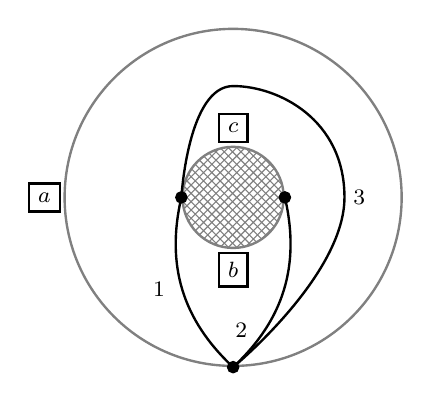
\begin{tikzpicture}[nodes={shape=circle,line width = 0.2ex, draw,font=\footnotesize},x=1ex,y=1ex, scale=2.5,baseline]
			\node[gray, inner sep=10ex] (an) {};
			\node[gray, pattern=crosshatch,pattern color=gray,inner sep=3 ex] at (an.center) (hole) {};
			\node[fill, inner sep=0.3ex] at (an.south) {};
			\node[fill, inner sep=0.3ex] at (hole.west) {};
			\node[fill, inner sep=0.3ex] at (hole.east) {};

			\uncover<2->{
				\draw (an.south) edge[bend left, line width = 0.2ex] node[draw=none, left] {1} (hole.west);
				\draw (an.south) edge[bend right, line width = 0.2ex] node[draw=none, left, near start] {2} (hole.east);
				\draw[line width = 0.2ex] plot [smooth, tension=1] coordinates {
						(an.south)
						($(hole.east) + (2,0)$) ($(hole.north) + (0,2)$)
						(hole.west)
					};
				\node[draw=none, left, outer sep=1.8ex] at (an.east) {3};

				\node[left, rectangle, outer sep=0.3ex] at (an.west) {$a$};
				\node[below, rectangle, outer sep=0.3ex] at (hole.south) {$b$};
				\node[above, rectangle, outer sep=0.3ex] at (hole.north) {$c$};
			}
		\end{tikzpicture}
		\uncover<3>{
			$\quad \longrightarrow \quad$
			\begin{tikzcd}[column sep=small,ampersand replacement=\&, arrows={-Latex, line width = 0.2ex}]
				\boxed{a} \ar[rr, -Latex, line width = 0.2ex] \& \& 3 \drar \dlar \& \& \boxed{c} \ar[ll] \\
				\& 1 \ular \drar \& \& 2 \ar[ll] \urar \& \\
				\& \& \boxed{b} \urar \& \&
			\end{tikzcd}
		}
	\end{center}
\end{frame}

\section{Algebra $\to$ combinatorics}

\begin{frame}
	\frametitle{Other objects with cluster structure}

	\begin{itemize}
		\item $X$ algebraic variety = set of zeros of a system of polynomials
		\item e.g. $X$ is a circle, a line, a torus, a plane, ... \pause
		\item $\mathbb{C}[X]$ coordinate algebra = polynomial functions on $X$.
	\end{itemize}
	\pause
	\textbf{Goal:} $\mathbb{C}[X] \cong$ cluster algebra
	\\
	$\leadsto$ Shows hidden combinatorial structure in $X$

\end{frame}

\begin{frame}
	\frametitle{Grassmannians}
	\begin{itemize}
		\item The Grassmannian $\Gr(d,n)$ = set of $d$-dimensional subspaces of $\bbC^n$
		\item For example, $\Gr(1, n) = \bbP(\bbC^n)$ (projective space)
	\end{itemize}
	\pause
	\begin{theorem}
		$\mathbb{C}[\Gr(2,n)] \cong $ cluster algebra of $n$-gon.
	\end{theorem}
	\pause
	Idea of proof:
	\begin{itemize}
		\item Write down relations in $\bbC[\Gr(2,n)]$
		\item Notice they are the same as Ptolomy's rule
		\item Finish by a dimension argument
	\end{itemize}

\end{frame}

\begin{frame}
	\frametitle{Canonical bases}

	\begin{itemize}
		\item $X = G$ algebraic group, e.g. $SL_n$.
	\end{itemize}
	\pause
	\begin{theorem}[Lusztig--Kashiwara '90]
		$\mathbb{C}[G]$ has very special type of linear basis: ``dual canonical/crystal basis''.
	\end{theorem}
	\pause
	Difficulties:
	\begin{itemize}
		\item Construction
		\item Multiplication rules for basis elements
	\end{itemize}
	\pause
	$\leadsto$ Want cluster algebra structure

\end{frame}

\section{Quantum cluster algebras}

\begin{frame}
	\frametitle{Shortcomings}

	Shortcomings:
	\begin{enumerate}
		\item Commutative, so not for quantum groups\\ \pause $\leadsto$ quantum cluster algebra,
		      i.e.,
		      \begin{equation*}
			      x_i x_j = q_{ij} x_j x_i
		      \end{equation*}%
		      \pause
		\item Case-by-case
	\end{enumerate}

\end{frame}

\begin{frame}
	\frametitle{Goodearl--Yakimov}

	\begin{center}
		``Quantum cluster algebra structures on quantum nilpotent algebras''
	\end{center}
	\begin{itemize}
		\item Paper by K. Goodearl and M. Yakimov (100+ pages)
		\item Part of a series of multiple papers
	\end{itemize}

\end{frame}

\begin{frame}
	\frametitle{CGL extensions}
	\begin{itemize}
		\item $A$ an algebra
		\item Ore extension $A[x; \sigma, \delta]$ is algebra such that
		      \begin{equation*}
			      x a = \sigma(a) x + \delta(a)
		      \end{equation*}
		\item CGL extension $\approx$ iterated Ore extension
		      \begin{equation*}
			      R = \bbC[x_1][x_2; \sigma_2, \delta_2][x_3; \sigma_3, \delta_3] \dotsb [x_N; \sigma_N, \delta_N]
		      \end{equation*}
	\end{itemize}
	\begin{theorem}[Goodearl--Yakimov, 2017]
		If $R$ is a CGL extension, then $R \cong$ quantum cluster algebra.
	\end{theorem}

\end{frame}

\begin{frame}
	\frametitle{Examples of CGL extensions}

	Some examples:
	\begin{itemize}
		\item $\bbC_q[M_{n\times m}]$: quantized matrix coordinate algebras
		\item $A^n_q(\bbC)$: quantized Weyl algebras
		\item More generally: $\mcU_q(\mfn_+ \cap w(\mfn_-))$ quantum Schubert cell algebras
		\item Double Bruhat cells \pause
		\item Heisenberg double: $\HeisUqn$
	\end{itemize}
	\medskip
	\pause
	Future: more general Heisenberg doubles

\end{frame}

\appendix

\section{Extra slides}

\begin{frame}
	\frametitle{Exchange graph}
	\begin{center}

		\resizebox{!}{0.95\textheight}{%
			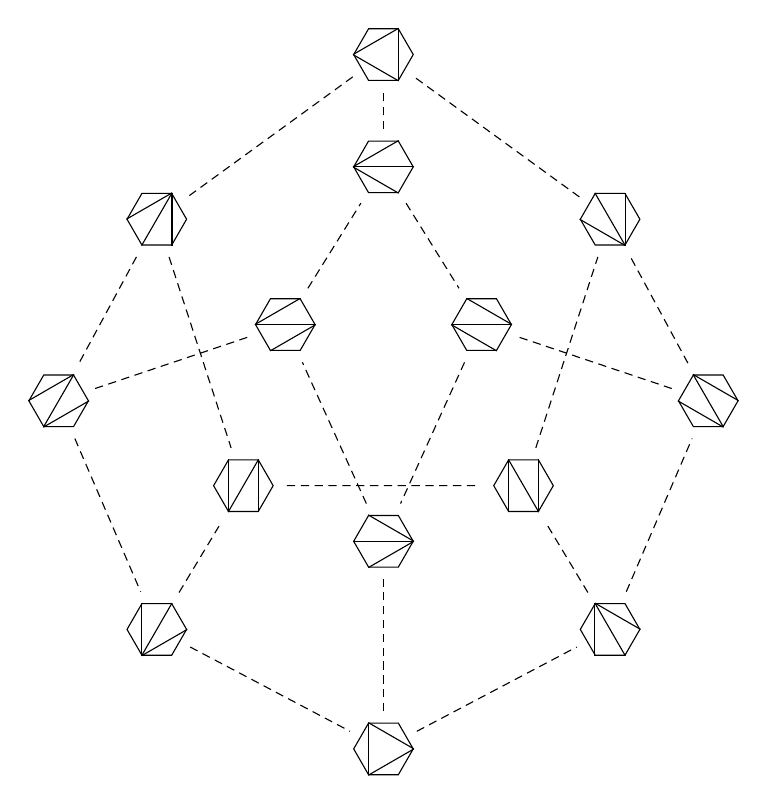
\begin{tikzpicture}[
					every node/.style={draw, minimum size = 5ex, shape=regular polygon, regular polygon sides =6},
				]
				\def\radius{20ex}
				\begin{scope}[rotate=90]
					\node[name=H1] at (0:\radius) {};
					\draw (H1.corner 3) -- (H1.corner 5);
					\draw (H1.corner 1) -- (H1.corner 3);
					\draw (H1.corner 1) -- (H1.corner 5);
					\node[name=H2] at (72:\radius) {};
					\draw (H2.corner 1) -- (H2.corner 3);
					\draw (H2.corner 1) -- (H2.corner 4);
					\draw (H2.corner 1) -- (H2.corner 5);
					\node[name=H3] at (144:\radius) {};
					\draw (H3.corner 2) -- (H3.corner 4);
					\draw (H3.corner 1) -- (H3.corner 4);
					\draw (H3.corner 1) -- (H3.corner 5);
					\node[name=H4] at (216:\radius) {};
					\draw (H4.corner 2) -- (H4.corner 4);
					\draw (H4.corner 2) -- (H4.corner 5);
					\draw (H4.corner 1) -- (H4.corner 5);
					\node[name=H5] at (288:\radius) {};
					\draw (H5.corner 3) -- (H5.corner 5);
					\draw (H5.corner 2) -- (H5.corner 5);
					\draw (H5.corner 1) -- (H5.corner 5);

					\node[name=H6, below=30ex of H2] {};
					\node[name=H7, below right=12ex and 5ex of H5] {};
					\node[name=H8, below left=12ex and 5ex of H2] {};
					\node[name=H9, below=5ex of H1] {};
					\node[name=H10, below=27ex of H9] {};
					\node[name=H11, below right=10ex and 5ex of H9] {};
					\node[name=H12, below left=10ex and 5ex of H9] {};
					\node[name=H13, below=13ex of H10] {};
					\node[name=H14, below=30ex of H5] {};

					\draw (H13.corner 2) -- (H13.corner 4);
					\draw (H13.corner 6) -- (H13.corner 4);
					\draw (H13.corner 6) -- (H13.corner 2);

					\draw (H14.corner 2) -- (H14.corner 4);
					\draw (H14.corner 2) -- (H14.corner 6);
					\draw (H14.corner 2) -- (H14.corner 5);

					\draw (H6.corner 2) -- (H6.corner 4);
					\draw (H6.corner 1) -- (H6.corner 4);
					\draw (H6.corner 6) -- (H6.corner 4);

					\draw (H8.corner 1) -- (H8.corner 3);
					\draw (H8.corner 1) -- (H8.corner 4);
					\draw (H8.corner 6) -- (H8.corner 4);

					\draw (H7.corner 3) -- (H7.corner 5);
					\draw (H7.corner 2) -- (H7.corner 6);
					\draw (H7.corner 2) -- (H7.corner 5);

					\draw (H9.corner 3) -- (H9.corner 5);
					\draw (H9.corner 1) -- (H9.corner 3);
					\draw (H9.corner 3) -- (H9.corner 6);

					\draw (H11.corner 3) -- (H11.corner 5);
					\draw (H11.corner 2) -- (H11.corner 6);
					\draw (H11.corner 3) -- (H11.corner 6);

					\draw (H12.corner 4) -- (H12.corner 6);
					\draw (H12.corner 1) -- (H12.corner 3);
					\draw (H12.corner 3) -- (H12.corner 6);

					\draw (H10.corner 3) -- (H10.corner 6);
					\draw (H10.corner 6) -- (H10.corner 4);
					\draw (H10.corner 6) -- (H10.corner 2);

					% Fake nodes to have some padding. 
					% Can't set outer sep on original nodes because it messes up the diagonals.
					\begin{scope}[nodes={draw=none, outer sep = 1ex}]
						\foreach \x in {1,...,14} {\node[name=H\x'] at (H\x) {};}
					\end{scope}

					\begin{scope}[every path/.style={densely dashed}]
						\draw (H1') -- (H2') -- (H3') -- (H4') -- (H5') -- (H1');
						\draw (H2') -- (H8') -- (H6') -- (H13') -- (H14') -- (H7') -- (H5');
						\draw (H9') -- (H11') -- (H10') -- (H12') -- (H9');
						\draw (H9') -- (H1');
						\draw (H8') -- (H12');
						\draw (H7') -- (H11');
						\draw (H6') -- (H3');
						\draw (H14') -- (H4');
						\draw (H13') -- (H10');
					\end{scope}
				\end{scope}
			\end{tikzpicture}
		}%
	\end{center}
\end{frame}

\end{document}